\documentclass[12px]{article}
\usepackage{graphicx} % Required for inserting images

\usepackage[T2A]{fontenc}
\usepackage[utf8]{inputenc}
\usepackage[english, russian]{babel}
\usepackage{amsmath}

\usepackage{geometry}
 \geometry{
 a4paper,
 total={170mm,257mm},
 left=20mm,
 top=20mm,
 }

\title{ЭВМ}
\author{VG6}

\begin{document}

\maketitle

\section{До этого мне было лень}
\section*{Вопросики (23 октября 2025)}
Какой принцип Неймана позволяет привесить скорость света?\\
Вычислительный процесс следует организовывать параллельным образом.\\
Почему ЭВМ в двоичной системе счисления, а не в десятичной?\\
5 принцип Неймана: разработка устройств для других операция нецелесообразно (кроме сумматора). В теории он прав, а на практике нет. К примеру аппаратные умножители. \\
\textbf{Главный принцип Неймана}: и программа и данные лежат в одном и том же месте в одном и том же виде. Не нужно для заменять машину, можно заменить только программу. \\
\textbf{Схема} - графическое обозначение элементов и связи между ними. \\

\section{Структура классической ЭВМ.}
Состоит из 3х блоков.\\
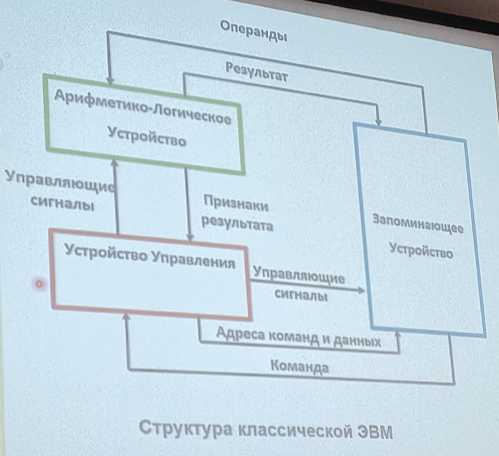
\includegraphics[width=0.5\linewidth]{images/Схема ЭВМ.png}\\
\subsection{Описание блоков.}
\begin{enumerate}
    \item Арифметико-Логическое устройство
    \begin{itemize}
        \item Выполняет преобразование информации представленной в двоичном виде. Например: числа при выполнении арифметической операции. 
        \item \textbf{Операнд} - мы будем называть участника арифметической или логической операции. 
        \item АЛУ преобразует операнды и получает результат и признаки результат (дополнительные сведенья о том, какй результат получился Правильный/Неправильный).
        \item Какой операцией заняться определяют управляющие сигналы.
        \item \textbf{Операция} - арифметическое или логическое действие выполняемое в АЛУ над операндами. То, что может делать АЛУ называется операцией.
    \end{itemize}
    \item Запоминающее устройство
    \begin{itemize}
        \item Предназначение: хранить двоичные числа.\\
        Для этого нужны 3 операции:
        \begin{enumerate}
            \item Запись
            \item Чтение
            \item Выборка (адресация не совсем одно и тоже)
        \end{enumerate}
        \item Запоминающее устройство классической ЭВМ является адресным устройством. Каждое число хранится в ячейке имеющей свой уникальный адрес, который тоже является числом. В простейшем случае - порядковый номер ячейки памяти.
        \item Запоминающее устройство представляет собой одномерный массив, где в качестве индекса выступает адрес (номер ячейки).
        \item 4 действия (тоже + хранение) определяется управляющими сигналами, среди которых сигналы: операции записи, чтения и многое другое. 
    \end{itemize}
    \item Устройство Управления
    \begin{itemize}
        \item Занимается управлением вычислительным процессом. Тоесть его выходом является порождение управляющих сигнаов (сигналов управления), которые потребляются другими ящиками и самим собой. 
        \item Помимо внешних блоков он управляет и самим собой.
        \item Цели и задачи управления: реализация выполнения команды. Для этого формируемые им сигналы несут 2 сущности: что делать, когда это надо сделать.
        \item Эту команду откуда-то надо взять. А они лежат в запоминающем устройстве, там же, где и данные. 
        \item На выходе сигналы, на входе ... из памяти
        \item нужно формировать адресс ячейки откуда взять команду, получить её и выполнить.
    \end{itemize}
\end{enumerate}
Связи между этими блоками изображены на рисунке.
По признакам результата УУ влияет на дальнейшее прохождение вычислительного процесса (изменять последовательность выполнения команд).\\\\
Например, произошло переполнение, значит нужно сформировать признак переполнения и передать УУ.\\\\
УУ получает команды из памяти, однако и операнды и команды лежат в разных ячейках запоминающего устройства (адресам) поэтому УУ должен формировать адреса как команд, так и операнд.
\subsection{Цикл выполнения команды.}
Структура организована циклически. И этот бег по кругу является бесконечным повторением. \\

\subsection{Память. Запоминающее устройство.}
Строится по иерархическому приципу.
\textbf{Регистр} - запоминающее устройство ёмкостью в 1 число. Есть 2 типа:
\begin{enumerate}
    \item Специальзированные регистры, функции которых предопределены конструкцией ЭВМ и являются неизменными и регистры 
    \item Общего назначения, функционал которых может предопределятся. Доступны для программистов.
\end{enumerate}
\subsubsection{Виды памяти}
\textbf{Сверхоперативные ЗУ} - обычно безадресного типа. К таким устройствам относятся буферные запоминающие устройства, стек.\\
\textbf{Буфер} - запоминающее устройство между ЗУ с разной скоростью работы для сглаживаний по времени. Обычно организуется очередью (FIFO).\\
\textbf{Стек} - первым вылетает последний заряженный патрон. (LIFO). История перехода к подпрограммам. Используется в системе прерываний.\\
\textbf{Постоянное запоминающее устройство (ROM)} - адресное запоминающее устройство без функции записи.
\textbf{EPROM} - оставляет возможность сменить содержимое путём перезаписи, что требует специальное устройство (программатор).\\
\textbf{КЭШ L1, L2, L3, L4} - безадрессное ассоциативное запоминающее устройство. Небольшая ёмкость, но кратно ускоряет скорость работы вычислительного устройства. Благодаря ассоциативному доступу (тэгами) аккумулируют в себе те команды или данные, которые используются наиболее интенсивно. Тем самым создавая копию ячеек Оперативной памяти кратно уменьшают доступ к этим данным.\\
\textbf{\textit{Основная оперативна память ООП}, ОЗУ, RAM, память с произвольной выборкой, память ЭВМ} - (синенькое на схеме) память, в которой хранятся те самые команды и данные по Нейману.\\
\textbf{Специализированные блоки памяти} - обмен между вычислительным ядром внешним миром (многопортовая память, ассоциативные ЗУ (используется в КЭШе и т.д. при поиске не по адресу, а по признаку), видеопамять)\\
\textbf{Внешние запоминающие устройства} - то, что подключается к ... через интерфейс. (..., облачные зранилища, Data-центры, ...)

\subsection{ОЗУ. Оперативное запоминающее устройтсво.}
Совокупность ячеек, пре
данный вид памяти для работы в качестве основной опреративной памяти ЭВМ дляжно обладать свойством произвольной выборки. \\

\textbf{Памятью с произвольной выборкой} мы будем называть адресное ЗУ, время выборки которого не зависит от адреса ячейки и последовательности обращений к ячейкам этого устройства.\\

Технические характеристики ЗУ: 
\begin{itemize}
    \item 1 бит - 1 двоичный разряд
    \item 1 байт - 8 бит. Попытка представить символы алфавита при помощи таблички кодирования (ASCII).
    \item К(Кило) - $2^{10} = 1024$
    \item М(Мега) - $2^{20} = ... $ 
    \item Г(Гига) - $2^{30} = ... $
\end{itemize}

\textbf{Память} - информационная ёмкость 1 адресуемой ячейки того, что имеет адрес. \\

\textbf{Организация ЗУ} - произведение числа ячеек на их разрядность, например: 4Гx8\\
Характеристики запоминающего устройства - временные.\\

\textbf{Быстродействие (производительность) ЗУ} - оценивают временами считывания и записи, длительностью циклов считывания/записи

\textbf{Время считывания} — интервал времени между моментом сигнала на считывание (адрес или разрешение считывания) и моментом выдачи данных на выходы памяти.

\textbf{Время записи} - интервал времени после задания сигнала записи, достаточный для установления ячейки в состояние, задаваемое входными данными.

\textbf{Цикл считывания/записи} - минимальный интервал между последовательными обращениями.
\subsection{Примеры условных графических обозначений (УГО ЗУ)}
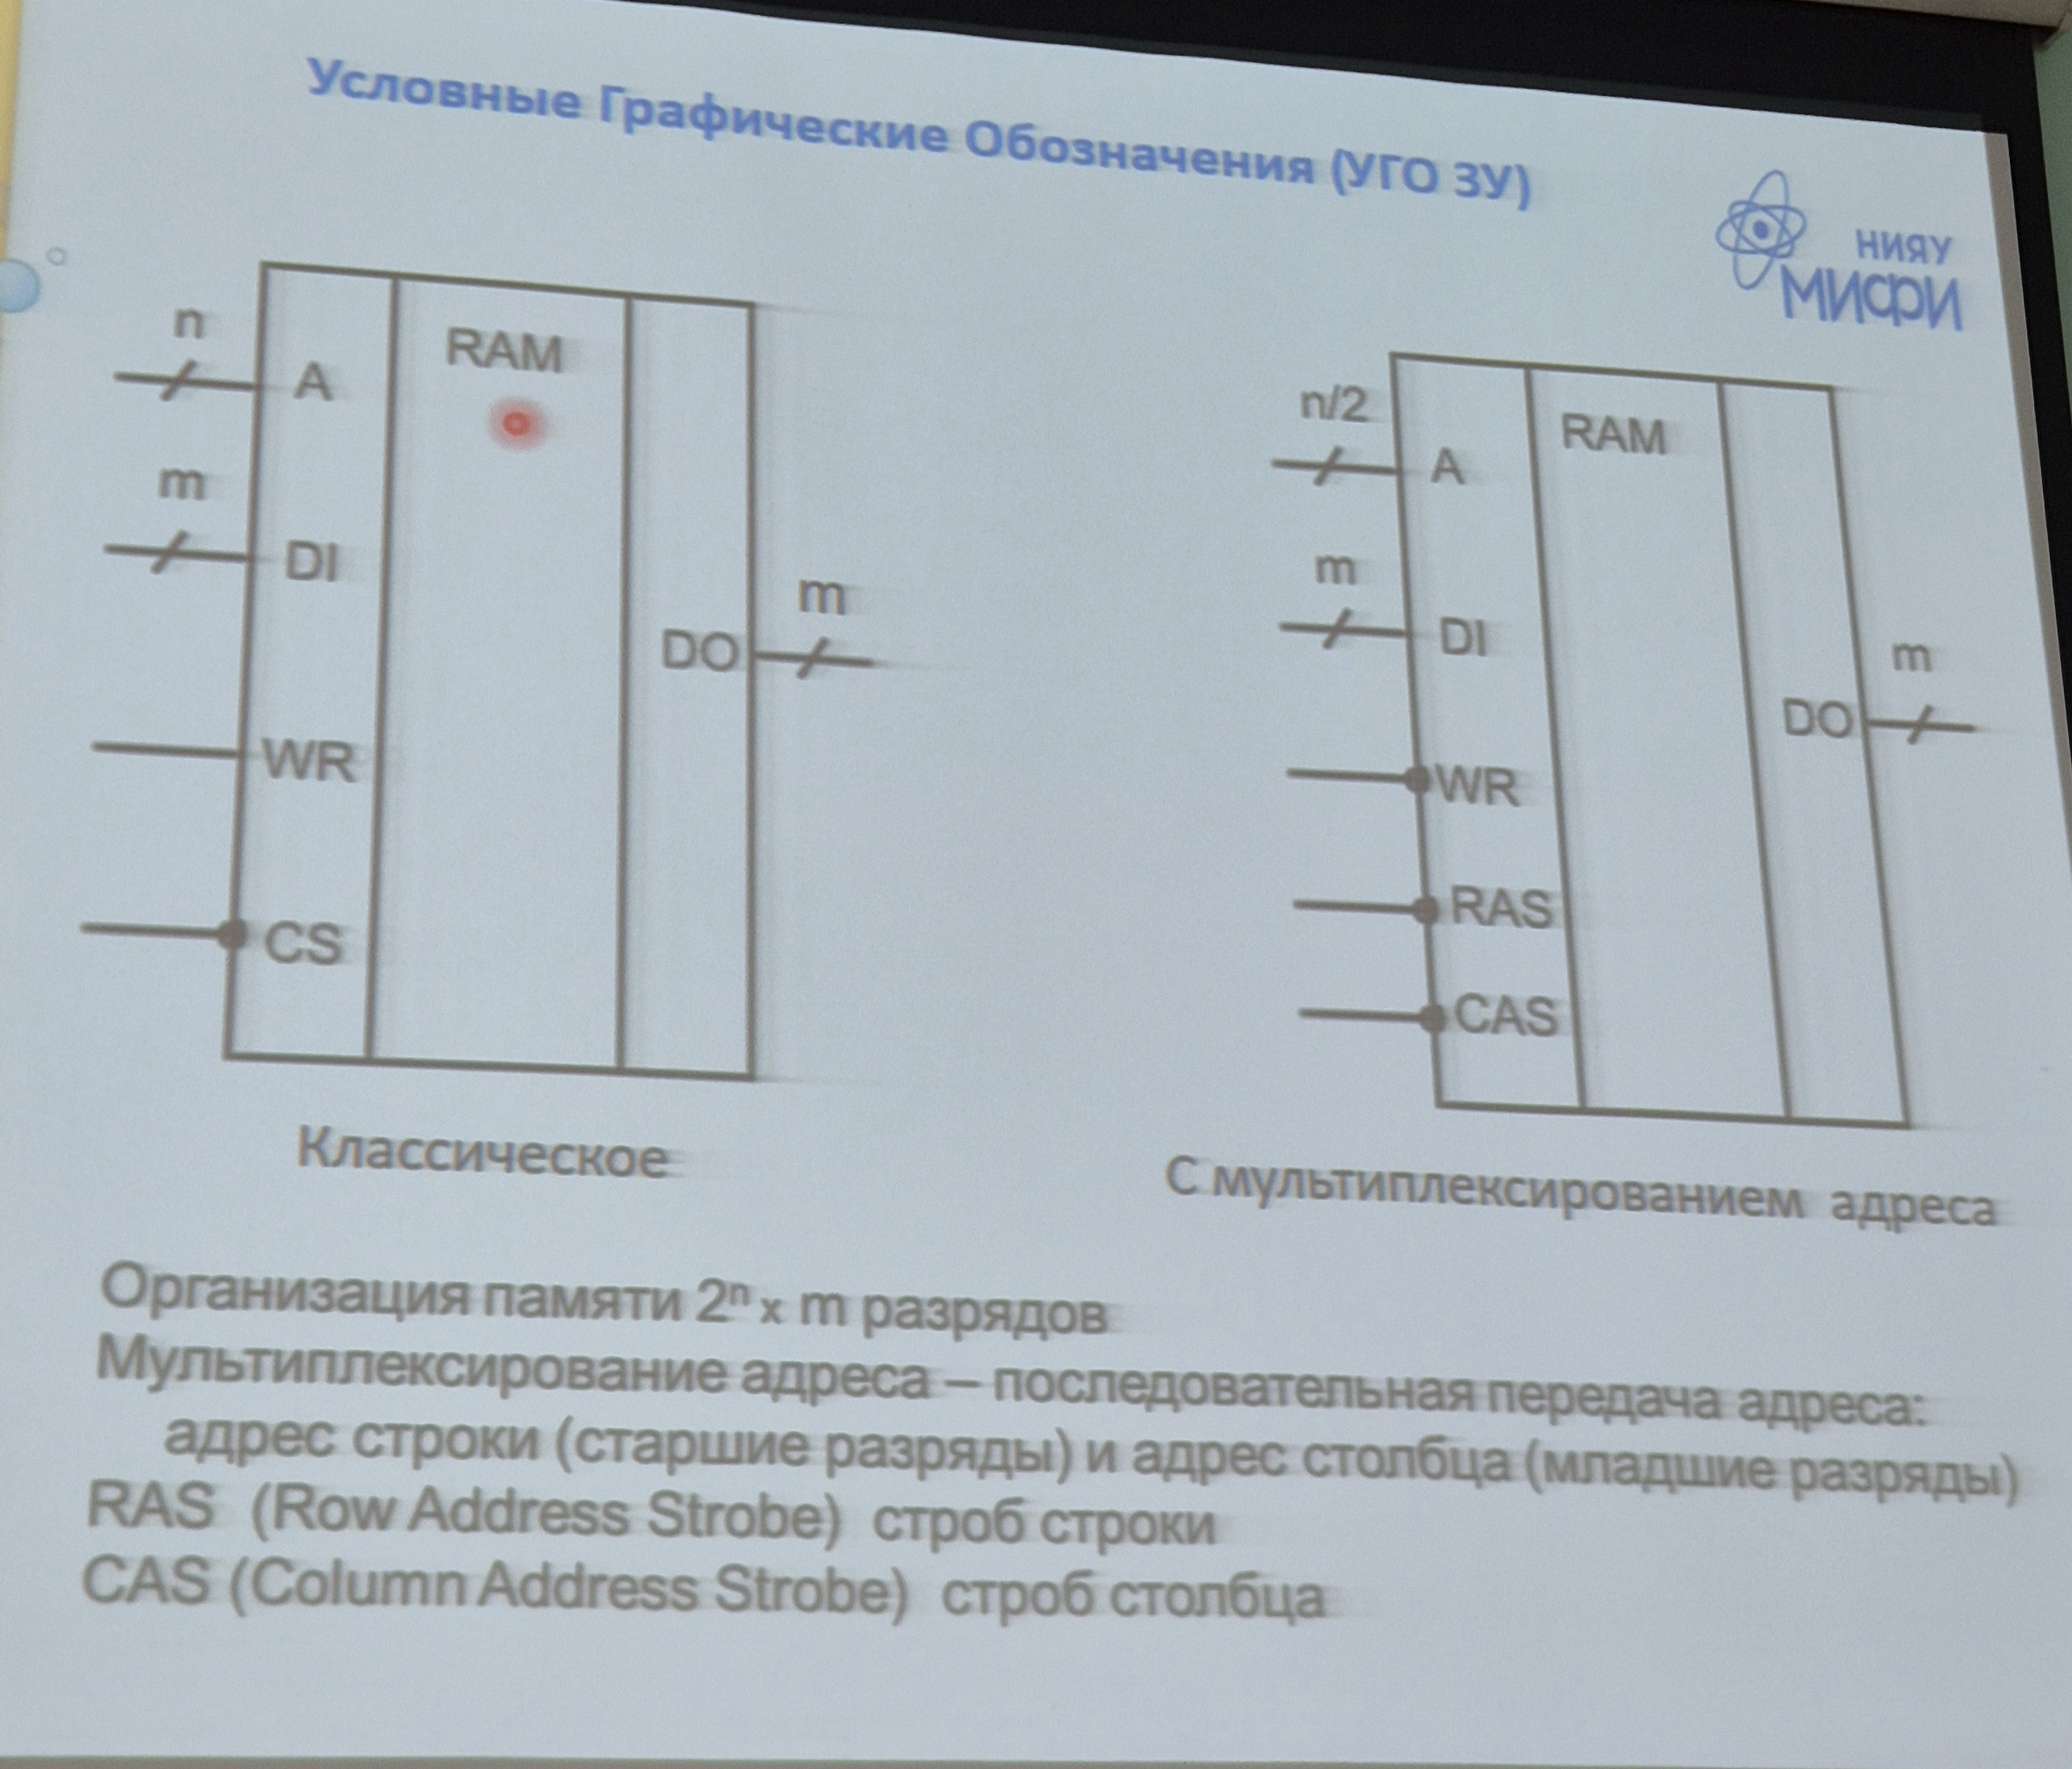
\includegraphics[width=0.5\linewidth]{images/УГО ЗУ.jpg}\\
\textbf{n} - разрядность шины адреса (количество проводов). \\
\textbf{A} - адрес.\\
\textbf{DI} - Data Input. m - размер слова этого запоминающего устройства.\\
\textbf{WR} - Write Read. Какую операцию выполнять\\
\textbf{CS} - Chin Select. Вход разрешения работы этого модуля. Если на схеме выколотая точка, то это означает, что разрешающий сигнал "0".

Организация памяти: $2^n * m$

\newpage
\setcounter{secnumdepth}{1}
\begin{center}
	\textbf{Семинары}
\end{center}

\section{Неопределённые функции}
Доопределять надо так, чтобы получился лучший результат. Для ДНФ доопределяем единицами, чтобы результат был короче. Для КНФ - нулями.
3 этапа:
\begin{enumerate}
	\item Доопределение
	\item Минимизация
	\item Коррекция		
\end{enumerate}

Алгоритм минимизации существует в 2 вариантах и содержат оба варианта все 3 этапа.\\
Вариант 1. 
\begin{itemize}
	\item Вводитяс вспомогательная функция \tilde{f} совпадающая с исходной на тех наборах на которых функция определена и принимающая значение 1 на запрещённых наборах.
	\item Выполняется минимизацию вспомогательной функции любым удобным способом.
	\item Строится импликантная матрица. Заголовками солбцов которой являются термы исходной функции, а заголовками строк - терми, полученные в результате минимизации вспомогательной функции. Проставляются метки, отмечающие вхождение строки в столбец и выбирается такая миимальная совокупность столбцов и строк, которая покроет всю функцию.
\end{itemize}
Вариант 2
\begin{itemize}
	\item Вводится вспомогательная функция $\tilde{f}$ которая совпадает с исх функцией на наборах, где она определена и принимает знаение 0 на запрещённых наборах.
	\item Выполняется минимизацию вспомогательной функции любым удобным способом.
	\item Строится импликантная матрица. Заголовками солбцов которой являются термы исходной функции, а заголовками строк - термы, полученные в результате минимизации вспомогательной функции. Проставляются метки, отмечающие вхождение строки в столбец и выбирается такая миимальная совокупность покрывающая все столбцы.
\end{itemize}

Условные обозначения
$ f(a, b, c) = \begin{cases}
	\sum_1 (1, 2, 3)\\
	X(4, 5)$ - запрещённые наборы$
\end{cases} $
\subsubsection*{Пример}
$ f(a, b, c, d) = \begin{cases}
	\sum_1(0, 5, 8, 12, 15), \\
	X (1, 2, 3, 10, 13, 14)
\end{cases}  \Rightarrow$
$\tilde{f} (a, b, c, d) = \begin{cases}
	\sum_1(0, 5, 8, 12, 15, 
	1, 2, 3, 10, 13, 14)
\end{cases} $\\

\begin{tabular}{c c c c c c}
	& b & b & \overline{b} & \overline{b} & \\
	a & 1 & 1 &   & 1 & \overline{c}\\
	a & 1 & 1 &   & 1 & c\\
	\overline{a} &   &   & 1 & 1 & c\\
	\overline{a} &   & 1 & 1 & 1 & \overline{c}\\
	 & \overline{d} & d & d & \overline{d}
\end{tabular}\\
\[ f(a, b, c, d) = ab + \overline{a}\overline{b} + \overline{b}\overline{d} + \overline{a}\overline{c}\overline{d} \]
\begin{tabular}{c c c c c c}
	 & 0000 & 0101 & 1000 & 1100 & 1111\\
	11-- &  & & & x & x \\
	00-- & x & & &  &  \\
	-0-0 & x &  & x &  \\
	0-01 &  & x & &  &  \\	
\end{tabular}
\[ bd + \overline{a}\overline{c}d + ab \]

\subsubsection*{Пример (минКНФ)}
$ f(a, b, c, d) = \begin{cases}
	$П$(3, 6, 7, 9, 11), \\
	X (0, 1, 2)
\end{cases}  \Rightarrow$
$ \tilde{f}(a, b, c, d) = \begin{cases}
	$П$(3, 6, 7, 9, 11, 0, 1, 2)
\end{cases} \\
\begin{tabular}{c c c c c c}
	   			  & b & b & \overline{b} & \overline{b} & \\
				a &   &   & 0 &   & \overline{c}\\
				a &   &   & 0 &   & c\\
	\overline{a}		  & 0 & 0 & 0 & 0 & c\\
	\overline{a} 		  &   &   & 0 & 0 & \overline{c}\\
	                          & \overline{d} & d & d & \overline{d}\\
\end{tabular}\\

\[ (a + \overline{c}) \cdot (b + \overline{d}) \cdot ab \]
\begin{tabular}{c c c c c c}
	     & 0011 & 0110 & 0111 & 1001 & 1011\\
	0-1- &  x   &  x   &  x   &      &     \\
	-0-1 &  x   &      &      &  x   &  x  \\
	00-- &  x   &      &      &      &     \\
\end{tabular}
\[ (a+\overline{c}) \cdot (b + \overline{d}) \]

\end{document}

